% taxonomy.tex — Task taxonomy diagram for TinkerRL Benchmark
% Standalone TikZ figure; can also be \input{} into main.tex
% Compile: pdflatex taxonomy.tex
\documentclass[tikz,border=4pt]{standalone}

\usepackage{tikz}
\usepackage{amssymb}  % for \checkmark
\usetikzlibrary{arrows.meta, positioning, shapes.geometric, calc, fit}

% ── Shared colour palette ────────────────────────────────────────────────────
\definecolor{RootBlue}    {RGB}{30,  90, 160}
\definecolor{MidBlue}     {RGB}{70, 140, 210}
\definecolor{LeafGreen}   {RGB}{ 55, 150,  90}
\definecolor{LeafBg}      {RGB}{220, 245, 228}
\definecolor{MidBg}       {RGB}{210, 232, 255}
\definecolor{RootBg}      {RGB}{180, 215, 255}
\definecolor{BadgeBg}     {RGB}{245, 245, 245}
\definecolor{ArrowGray}   {RGB}{100, 110, 125}

% ── Node styles ─────────────────────────────────────────────────────────────
\tikzset{
  % Root node
  root/.style={
    rectangle, rounded corners=6pt,
    fill=RootBg, draw=RootBlue, line width=1.2pt,
    text=RootBlue, font=\bfseries\small,
    inner sep=6pt, minimum width=3.2cm, minimum height=0.65cm,
    align=center
  },
  % Category (mid-level) nodes
  category/.style={
    rectangle, rounded corners=5pt,
    fill=MidBg, draw=MidBlue, line width=0.9pt,
    text=MidBlue, font=\bfseries\scriptsize,
    inner sep=5pt, minimum width=2.6cm, minimum height=0.58cm,
    align=center
  },
  % Leaf (task) nodes
  leaf/.style={
    rectangle, rounded corners=4pt,
    fill=LeafBg, draw=LeafGreen, line width=0.8pt,
    text=black, font=\scriptsize,
    inner sep=4pt, minimum width=2.4cm, minimum height=0.52cm,
    align=center
  },
  % Badge showing model count / status
  badge/.style={
    rectangle, rounded corners=2pt,
    fill=BadgeBg, draw=ArrowGray!60, line width=0.5pt,
    text=ArrowGray, font=\tiny,
    inner sep=2pt
  },
  % Arrow style
  treearrow/.style={
    ->, >=Stealth, line width=0.7pt, color=ArrowGray, rounded corners=3pt
  }
}

\begin{document}
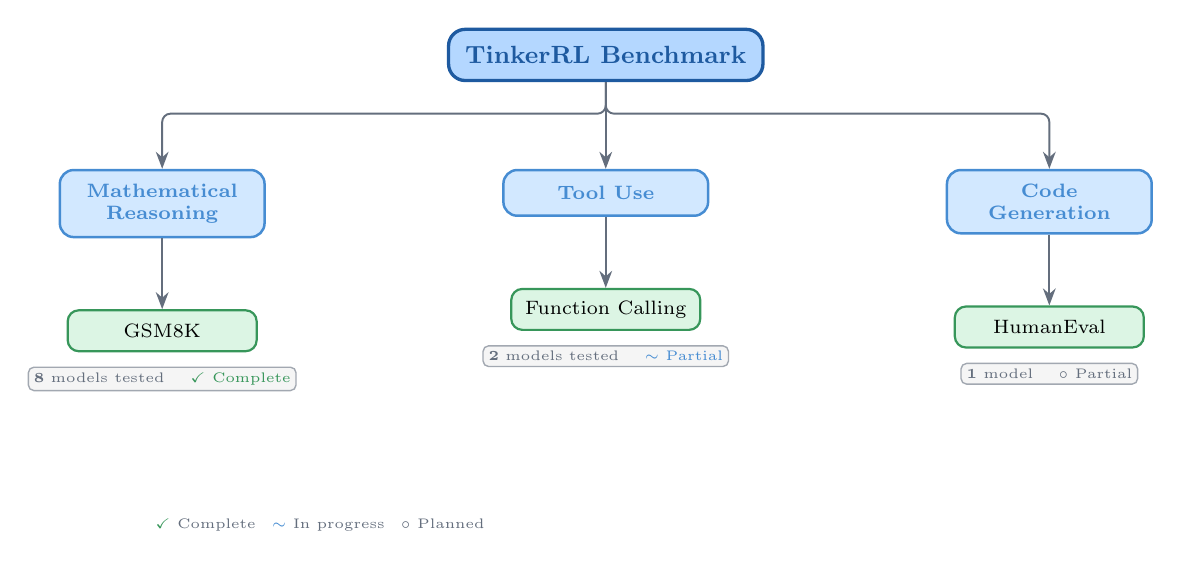
\begin{tikzpicture}[node distance=0.5cm and 1.0cm]

  % ── Root ──────────────────────────────────────────────────────────────────
  \node[root] (root) {TinkerRL Benchmark};

  % ── Category nodes (placed below root with horizontal spread) ─────────────
  \node[category, below left=1.1cm and 2.3cm of root]  (math)  {Mathematical\\Reasoning};
  \node[category, below=1.1cm of root]                  (tool)  {Tool Use};
  \node[category, below right=1.1cm and 2.3cm of root] (code)  {Code\\Generation};

  % ── Leaf nodes ────────────────────────────────────────────────────────────
  % Math → GSM8K
  \node[leaf, below=0.9cm of math] (gsm8k) {GSM8K};
  \node[badge, below=0.18cm of gsm8k] (gsm8k_badge)
        {\textbf{8} models tested \quad \textcolor{LeafGreen}{$\checkmark$ Complete}};

  % Tool → Function Calling
  \node[leaf, below=0.9cm of tool] (fc) {Function Calling};
  \node[badge, below=0.18cm of fc] (fc_badge)
        {\textbf{2} models tested \quad \textcolor{MidBlue}{$\sim$ Partial}};

  % Code → HumanEval
  \node[leaf, below=0.9cm of code] (he) {HumanEval};
  \node[badge, below=0.18cm of he] (he_badge)
        {\textbf{1} model \quad \textcolor{ArrowGray}{$\circ$ Partial}};

  % ── Edges: root → categories ──────────────────────────────────────────────
  \draw[treearrow] (root.south) -- ++(0,-0.4) -| (math.north);
  \draw[treearrow] (root.south) -- ++(0,-0.4) -| (tool.north);
  \draw[treearrow] (root.south) -- ++(0,-0.4) -| (code.north);

  % ── Edges: categories → leaves ────────────────────────────────────────────
  \draw[treearrow] (math.south) -- (gsm8k.north);
  \draw[treearrow] (tool.south) -- (fc.north);
  \draw[treearrow] (code.south) -- (he.north);

  % ── Legend ────────────────────────────────────────────────────────────────
  \node[font=\tiny, text=ArrowGray, align=left,
        below=1.5cm of gsm8k_badge, xshift=2.0cm]
  {%
    \textcolor{LeafGreen}{$\checkmark$} Complete \enspace
    \textcolor{MidBlue}{$\sim$} In progress \enspace
    \textcolor{ArrowGray}{$\circ$} Planned%
  };

\end{tikzpicture}
\end{document}
